\documentclass[10pt,a4paper]{book}
\usepackage[utf8]{inputenc}
\usepackage[T1]{fontenc}
\usepackage[english]{babel}
\usepackage{amsmath}
\usepackage{amsthm}
\usepackage{amsfonts}
\usepackage{amssymb}
\usepackage{graphicx}
\graphicspath{{images/}}
\author{Anirudh Gupta }
\title{Mathematics for Machine Learning}

\newtheorem{definition}{Definition}
\newtheorem{proposition}{Proposition}
\newtheorem{corollary}{Corollary}
\newtheorem{theorem}{Theorem}

\begin{document}
	\maketitle
	
		\chapter{Vector Spaces}
	
	A vector space is the general mathemtical structure we need to be able to talk about linear mappings. To introduce a vector space we need a lot of mathematical concepts. So we start with a group. 
	
	\begin{definition}
		A set $G$ of elements with an operation $+$: $G \times G \rightarrow G$ is called a group if the following properties hold: 
	\end{definition}
	
	\begin{itemize}
		\item[G1] Associativity: $ \forall a, b, c \in G$ : $(a + b) + c = a + (b + c) $
		\item[G2] Identity element: $\exists e \in G: \forall g \in G: e + g = g + e = g $
		\item[G3] Inverse element: $ \forall a \in G$, $ \exists b \in G : a + b = b + a = e$
	\end{itemize}
	
	A group is called a commutative group (Abelian group) if we have additionally that $ \forall a, b \in G: a + b = b + a$ \\
	
	\textbf{Examples}
	
	\begin{itemize}
		\item $(\Re^n, +)$: This can be thought of as an $n$-dimensional vector with addition as the associated operation. The addition of three vectors can be done in any order and is thus associative. The identity element in this case is the zero vector. The inverse element is the negative of each element. Thus this combination forms a group. 
		
		\item $(\Re^+, .)$: This is the set of positive real numbers with multiplication as the associated operation. This also forms a group. 
		
		\item $(\Re^-, .)$: This is set of negative real numbers with associated operation as multiplication. It does not form a group, since multiplication of two negative real numbers gives us a positive real number and that is out of the set considered. We can also say that the set of negative real numbers is not closed with respect to multiplication. 
		
	\end{itemize}

	\begin{definition}
		A set $F$ with two operation $ (+ , \cdot) : F \times F \rightarrow F$ is called a field if the following properties hold: 
	\end{definition}
	
	\begin{itemize}
		\item[F1] $ (F, +) $ is a commutative group with identity element 0.
		\item[F2] $(F \setminus\{0\}, \cdot)$ is a commutative group with identity element 1. 
		\item[F3] Distributivity:  $\forall a, b, c \in F: a \cdot (b + c) = a \cdot b + a \cdot c$
	\end{itemize}

	The two most common fields are the ral numbers $(\Re, +, \cdot)$ and complex numbers $(\mathbb{C}, +, \cdot)$ with defined addition and multiplication.
	
	\begin{definition}
		Let $F$ be a field with identity elements 0 and 1. A vector space over the field $F$ is a set $V$ with a mapping: $ (+) : V \times V \rightarrow V$ (vector addition)  and a mapping $(\cdot) : F \times V \rightarrow V$ (scalar multiplication) such that: 
	\end{definition}

	\begin{itemize}
		\item[V1] $(V, +)$ is a commutative group.
		\item[V2] Multiplicative identity: $\forall v \in V: 1 \cdot v = v$
		\item[V3] Distributive property: $\forall a, b  \in F$ and $ \forall u, v \in V$
			\subitem $a \cdot (u + v) = a \cdot u + a \cdot v$
			\subitem $(a + b)u = a \cdot u + b \cdot u $ 	
	\end{itemize}

	Elements of $V$ are called vectors and elements of $F$ are called scalars. Depending on whether the field is real or complex we call the space as real vector space or complex vector space. \\
	
	\textbf{Examples}
	
	\begin{itemize}
		
		\item $\Re^n$ with standard operations of adding vectors and multiplying vectors with a scalar. 
		\item Function spaces: These are spaces which consists of functions. And essentially the whole field of functional analysis exploits the fact if you group them in a vector space, there are many properties that you can find about functions without even explicitly looking at what type of functions you are talking about. 
		\subitem $\Re^\chi$ : $\{f: \chi \rightarrow \Re\}$ the space of all real valued functions on a set $\chi$. No we define the two operations: 
		\subitem $ + : \Re^\chi \times \Re^\chi \rightarrow \Re^\chi$ , $(f + g)(x) := f(x) + g(x)$
		\subitem $\cdot : \Re \times \Re^\chi \rightarrow \Re^\chi, (\lambda \cdot f)(x) := \lambda \cdot (f(x))$ \\
		Then $(\Re^\chi, +, \cdot)$ is a vector space.
	\end{itemize}
	\chapter{Basis and Dimension}

\begin{definition}
	Let $V$ be a vector space and $U \subset V$ a non-empty set. We call $U$ a subspace of $V$ if it is closed under linear combinations. \\
	$ \forall \lambda, \mu \in F$ and $\forall u, v \in V : \lambda u + \mu v \in U$, where $F$ is the field where scalars come from. 
\end{definition}

So essentially subspace is a vector space on its own. And it is closed means that we can add two elements and multiply by scalars and still remain in that space. \\

\textbf{Examples}

\begin{itemize}
	\item $C(\chi)$ is a subspace of $\Re^\chi$ where $C(\chi)$ is the set of continuous functions on domain $\chi$ and $\Re^\chi$ is any real valued function. Sum of two continuous functions is continuous and scalar multiplication of a continous function is a continous function as well. 
	\item The set $S$ of symmetric matrices of size $n \times m$ is a subspace of $\Re^{n \times m}$. Since sum of two symmetric matrices is a symmetric matrix and the same goes for scalar multiplication.  
\end{itemize}

\begin{definition}
	Let $V$ be a vector space over $F$ and $u_1,....,u_n \in V$, $\lambda_1,......\lambda_n \in F$. Then $\sum_{i=1}^{n} \lambda_i u_i$ is called a linear combination. The set of all linear combinations of $u_1,....,u_n$ is called the span (linear hull) of $u_1,....,u_n$. \\
	$span(u_1,....,u_n) := \{\sum_{i=1}^{n} \lambda_i u_i | \lambda_i \in F \}$  
\end{definition}

The set $U:= \{ u_1,....,u_n \}$ is the generator of $span(u_1,....,u_n)$

\begin{definition}
	A set of vectors $v_1,.....v_n$ is called linearly independent if the following holds: \\
	$ \sum_{i=1}^{n} \lambda_i v_i = 0 \implies \lambda_1 = ..... = \lambda_n = 0$ \\
\end{definition}

\textbf{Examples}

\begin{itemize}
	\item The vectors $\begin{bmatrix} 	1 \\ 0 \\ 0 \end{bmatrix}, \begin{bmatrix} 	2 \\ 1 \\ 0 \end{bmatrix}$ and $\begin{bmatrix} 3 \\ 4 \\ 1 \end{bmatrix} \in \Re^3$ are linearly independent. 
	\item The functions $sin(x)$ and $cos(x) \in \Re^\Re$ are linearly independent. 
	\item Any set of $d+1$ vectors in $\Re^d$ is linearly dependent.  
\end{itemize}

\begin{definition}
	A subset $B$ of a vector space $V$ is called a (Hammel) basis if: 
	\begin{itemize}
		\item $span(B) = V$
		\item $B$ is linearly independent. 
	\end{itemize}
\end{definition}

This means that any vector in $V$ can be written as a linear combination of vectoes in $B$ but basis vectors themselves cannot be written in terms of each other since they are independent. \\ 

\textbf{Examples}

\begin{itemize}
	\item The canonical basis of $\Re^3$ is  $\begin{bmatrix} 	1 \\ 0 \\ 0 \end{bmatrix}, \begin{bmatrix} 	0 \\ 1 \\ 0 \end{bmatrix}$ and $\begin{bmatrix} 0 \\ 0 \\ 1 \end{bmatrix}$.
	\item Another basis of $\Re^3$ is given by $\Re^3$ is  $\begin{bmatrix} 	1 \\ 0 \\ 0 \end{bmatrix}, \begin{bmatrix} 	1 \\ 1 \\ 0 \end{bmatrix}$ and $\begin{bmatrix} 1 \\ 1 \\ 1 \end{bmatrix}$. \\
\end{itemize}

\begin{proposition}
	If $U = \{u_1,....u_n\}$ spans a vector space $V$, then the set $U$ can be reduced to a basis of $V$.
\end{proposition}

\begin{proof}
	If $U$ is already linearly independent then we are done. If $U$ is linearly dependent, $ \exists u \in U$ that is a linear combination of other vectors in $U$. We repeat this step untill we reach a point where all vectors in $U$ are linearly independent. 
\end{proof}

\begin{definition}
	A vector space is called finite dimentional if it has a finite basis.
\end{definition}

\begin{proposition}
	Let $U = \{u_1,...,u_n\} \subset V$ be a set of linearly independent vectors and let $V$ be a finite dimensional vector space. Then $U$ can be extended to a basis of $V$. 
\end{proposition}

\begin{proof}
	Let $w_1,...,w_m$ be a basis of $V$. Consider a set $\{u_1,...u_n,w_1,...,w_m\}$. Remove vectors from the end untill remaining vectors are linearly independent. The remaining set $spans(V)$, is linearly independent by construction and contains $U$.
\end{proof}

\begin{corollary}
	Let $V$ be a finite dimensional vector space. Then any two basis of $V$ have the same length.
\end{corollary}

\begin{definition}
	The length of the basis of a finite dimensional vector space is called its dimension. 
\end{definition}

We have defined what a basis and we also know what a subspace is. Another notion which brings these two things together is known as the \textit{sum} and \textit{direct sum} of subspaces. 

\begin{definition}
	Assume that we have two subspaces $U_1$ and $U_2$ of a vector space $V$. The sum of the two spaces is defined as : \\
	$U_1 + U_2 := \{ u_1 + u_2 | u_1 \in U_1, u_2 \in U_2 \}$
\end{definition}

The sum which has just seen is known as the direct sum. If each element in the sum can be written in exactly one way$(U_1\oplus U_2)$.

\begin{proposition}
	Suppose $V$ is finite-dimensional, and $U \subset V$ is a subspace, then there exists a subspace $W \subset V$ such that $U \oplus W =  V$.
\end{proposition}

\begin{proof}
	Let the set $\{u_1,...u_k\}$ be a basis of $U$. Extend it to a basis of $V$, say the resulting set is $\{u_1,...u_k, v_1,...v_m\}$. Define $W = span\{v_1,...v_m\}$ 
\end{proof}

	\chapter{Linear Maps, Kernals and Range}

\begin{definition}
	Let $U$ and $V$ be vector spaces over the same field $F$. A mapping $T:U \rightarrow V$ is linear if 	$ \forall u_1, u_2 \in U, \forall \lambda \in F$ 
	\begin{center}
 		$T(u_1 + u_2) = T(u_1) + T(u_2)$\\ 
 		$T(\lambda u_1) = \lambda T(u_1)$
	\end{center}
	
\end{definition}

The set of all linear mappings from $U \rightarrow V$ is denoted by $\mathcal{L}(U,V)$. If $U=V$, then linear mappings are denoted by $\mathcal{L}(U)$, which is a set of linear mappings from a set onto itself. \\ 

\textbf{Examples}
\begin{itemize}
	\item $T: \mathcal{C}[a, b] \rightarrow \Re$, $f \rightarrow \int_{a}^{b} f(x) dx$. Integration is linear operator since it does not matter whether you add two functions and then integrate or vice versa. Also, we can pull out scalar multiples out of the integrals. 
	\item $D: \mathcal{C}^{\infty} [a, b] \rightarrow \mathcal{C}^{\infty} [a, b]$, $f \rightarrow f'$. The derivative of the sum of functions is the same as taking the sum and then derivatves. \\
\end{itemize}

\begin{definition}
	$T \in \mathcal{L}(U, V)$. Then the kernal of $T$ (null space) is defined as : 
	\begin{center}
		$ker(T) := null(T) := \{u \in U | Tu = 0\}$
	\end{center}
	
\end{definition}

\begin{proposition}
	$ker(T)$ is a subspace of $U$.
\end{proposition}

$T$ is injective iff $ker(T) = \{0\}$. Means if we take two input points in the input space then they are always mapped to different points in the output space. 
So 0 is always an element in the kernal since a linear map always maps 0 to 0. Thus the kernal is never empty. The smallest kernal of any vector space is just the 0 vector. 

\begin{definition}
	The range of $T$ (image of $T$) is defined as: 
	\begin{center}
		$range(T) := Image(T) := \{Tu | u \in U\}$
	\end{center}
\end{definition}

\begin{proposition}
	The range is always a subspace of $V$
\end{proposition}

$T$ is surjective iff $range(T) = V$

\begin{definition}
	$V' \subset V$ where $V'$ is any set. The pre-image of $V'$ is defined as: 
	\begin{center}
		$T^{-1} (V') := \{u \in U | Tu \in V'\}$
	\end{center} 
\end{definition}

\begin{proposition}
	If $V' \subset V$ is a subspace of V, then $T^{-1}(V')$ is a subspace of $U$.
\end{proposition}

\begin{figure}[h]
	\centering
	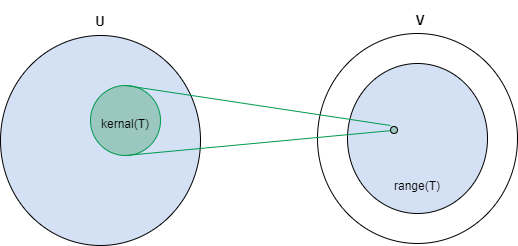
\includegraphics[width=0.5\textheight]{ch-3-img-1}
	\caption{Kernal and range of a $T: U \rightarrow V$}
\end{figure}

We can see in the figure above that a part of $U$ which is mapped to 0 is known as the kernal of tha map $T$. The range lives in $V$ and the kernal lives in $U$. 

\begin{theorem}
	Let $V$ be finite dimensionalm $W$ be any vector space and $T \in \mathcal{L}(V,W)$. Let $u_1,...,u_n$ be a basis of $ker(T) \subset V$. Let $w_1,...,w_m$ be a basis of the $range(T) \subset W$. Then $u_1,...,u_n$, $T^{-1}(w_1),...,T^{-1}(w_m)$ forms a basis of $V$. In particular , $dim(V) = dim(ker(T)) + dim(range(T))$
\end{theorem}

\begin{proof}
	Denote $T^{-1}(w_1) := z_1,...,T^{-1}(w_m) := z_m$. If $\{u_1,...u_n,z_1,...z_m\}$ for a basis of $V$, then they must span the whole space $V$ and be linearly independent. Let's do each step by step. \\
	Step 1: Prove that $V \subset span\{u_1,...u_n,z_1,...z_m\}$ \\ 
	Let $v \in V$, and $Tv \in range(T)$. Since we know the basis of $range(T)$,
	\begin{align*}
		\exists \lambda_1,...,\lambda_m: Tv &= \lambda_1 w_1 + ... + \lambda_m w_m \\
											&= \lambda_1 T(z_1) + ... + \lambda_m T(z_m) \\
											&= T(\lambda_1 z_1) + ... + T(\lambda_m z_m)
	\end{align*}
$ \implies Tv - T(\lambda_1z_1 + ... + \lambda_mz_m) = T(v - (\lambda_1z_1 + ... + \lambda_mz_m)) =  0$  \\
$\implies (v - (\lambda_1z_1 + ... + \lambda_mz_m)) \in kernal(T)$ since this vector is mapped to 0 by the linear mapping. Since we also know the basis of the kernal any vector in the kernal can be written as: 
\begin{align*}
(v - (\lambda_1z_1 + ... + \lambda_mz_m)) &= \mu_1 u_1 + ... + \mu_n u_n \\ 
v &= \lambda_1 z_1 + ... + \lambda_m z_m + \mu_1 u_1 + ... + \mu_n u_n
\end{align*}
Step 2 : Prove that $u_1,...,u_n, z_1,...,z_m$ are linearly independent. \\ 
Assume that $\mu_1 u_1 + ... \mu_n u_n + \lambda_1 z_1 + ... + \lambda_m z_m  = 0$ \\
If these vectors are linearly independent then all the coefficients will simultaneously go to zero. 
\begin{align*}
	\lambda_1 w_1 + ... + \lambda_m w_m &= \lambda_1 T(z_1) + ... + \lambda_m T(z_m) \\
	&= \lambda_1 T(z_1) + ... + \lambda_m T(z_m) + \mu_1 T(u_1) + ... + \mu_n T(u_n) \\ 
	&= T(\lambda_1 z_1 + ... \lambda_m z_m + \mu_1 u_1 + ... + \mu_n u_n) = T(0) = 0
\end{align*}
We can add $ \mu_1 T(u_1) + ... + \mu_n T(u_n)$ to the expression since it goes to zero by definition of a kernal. Everything inside the operator is zero due to the assumption at the beginning of step 2. 
Since $\lambda_1 w_1 + ... + \lambda_m w_m = 0$ and $w_1,...,w_m$ is a basis 
$\implies \lambda_1 = ... = \lambda_m = 0$ \\
Now $\mu_1 u_1 + ... + \mu_n u_n = 0$ since we have already proved the other half of the assumption to be zero. Since $u_1,...,u_n$ is the basis of the kernal $\implies \mu_1=...\mu_n=0$.
\end{proof}

\begin{proposition}
	Let $T \in \mathcal{L}(V, W)$ and $V, W$ be finite dimensional, then the following statements are equivalent.
	\begin{itemize}
		\item T is injective
		\item T is surjective
		\item T is bijective
	\end{itemize} 
\end{proposition}

This proposition does not hold in infinite dimensional spaces. 




	 
\end{document}